\subsection{Задача $3 \times 2$}

На следующем рисунке показано допусковое множество решений для задачи $3 \times 2$. Кроме того, показан квадрат с центром в точке максимума распознающего функционала ширины ive:

\begin{figure}[H]
	\begin{center}
		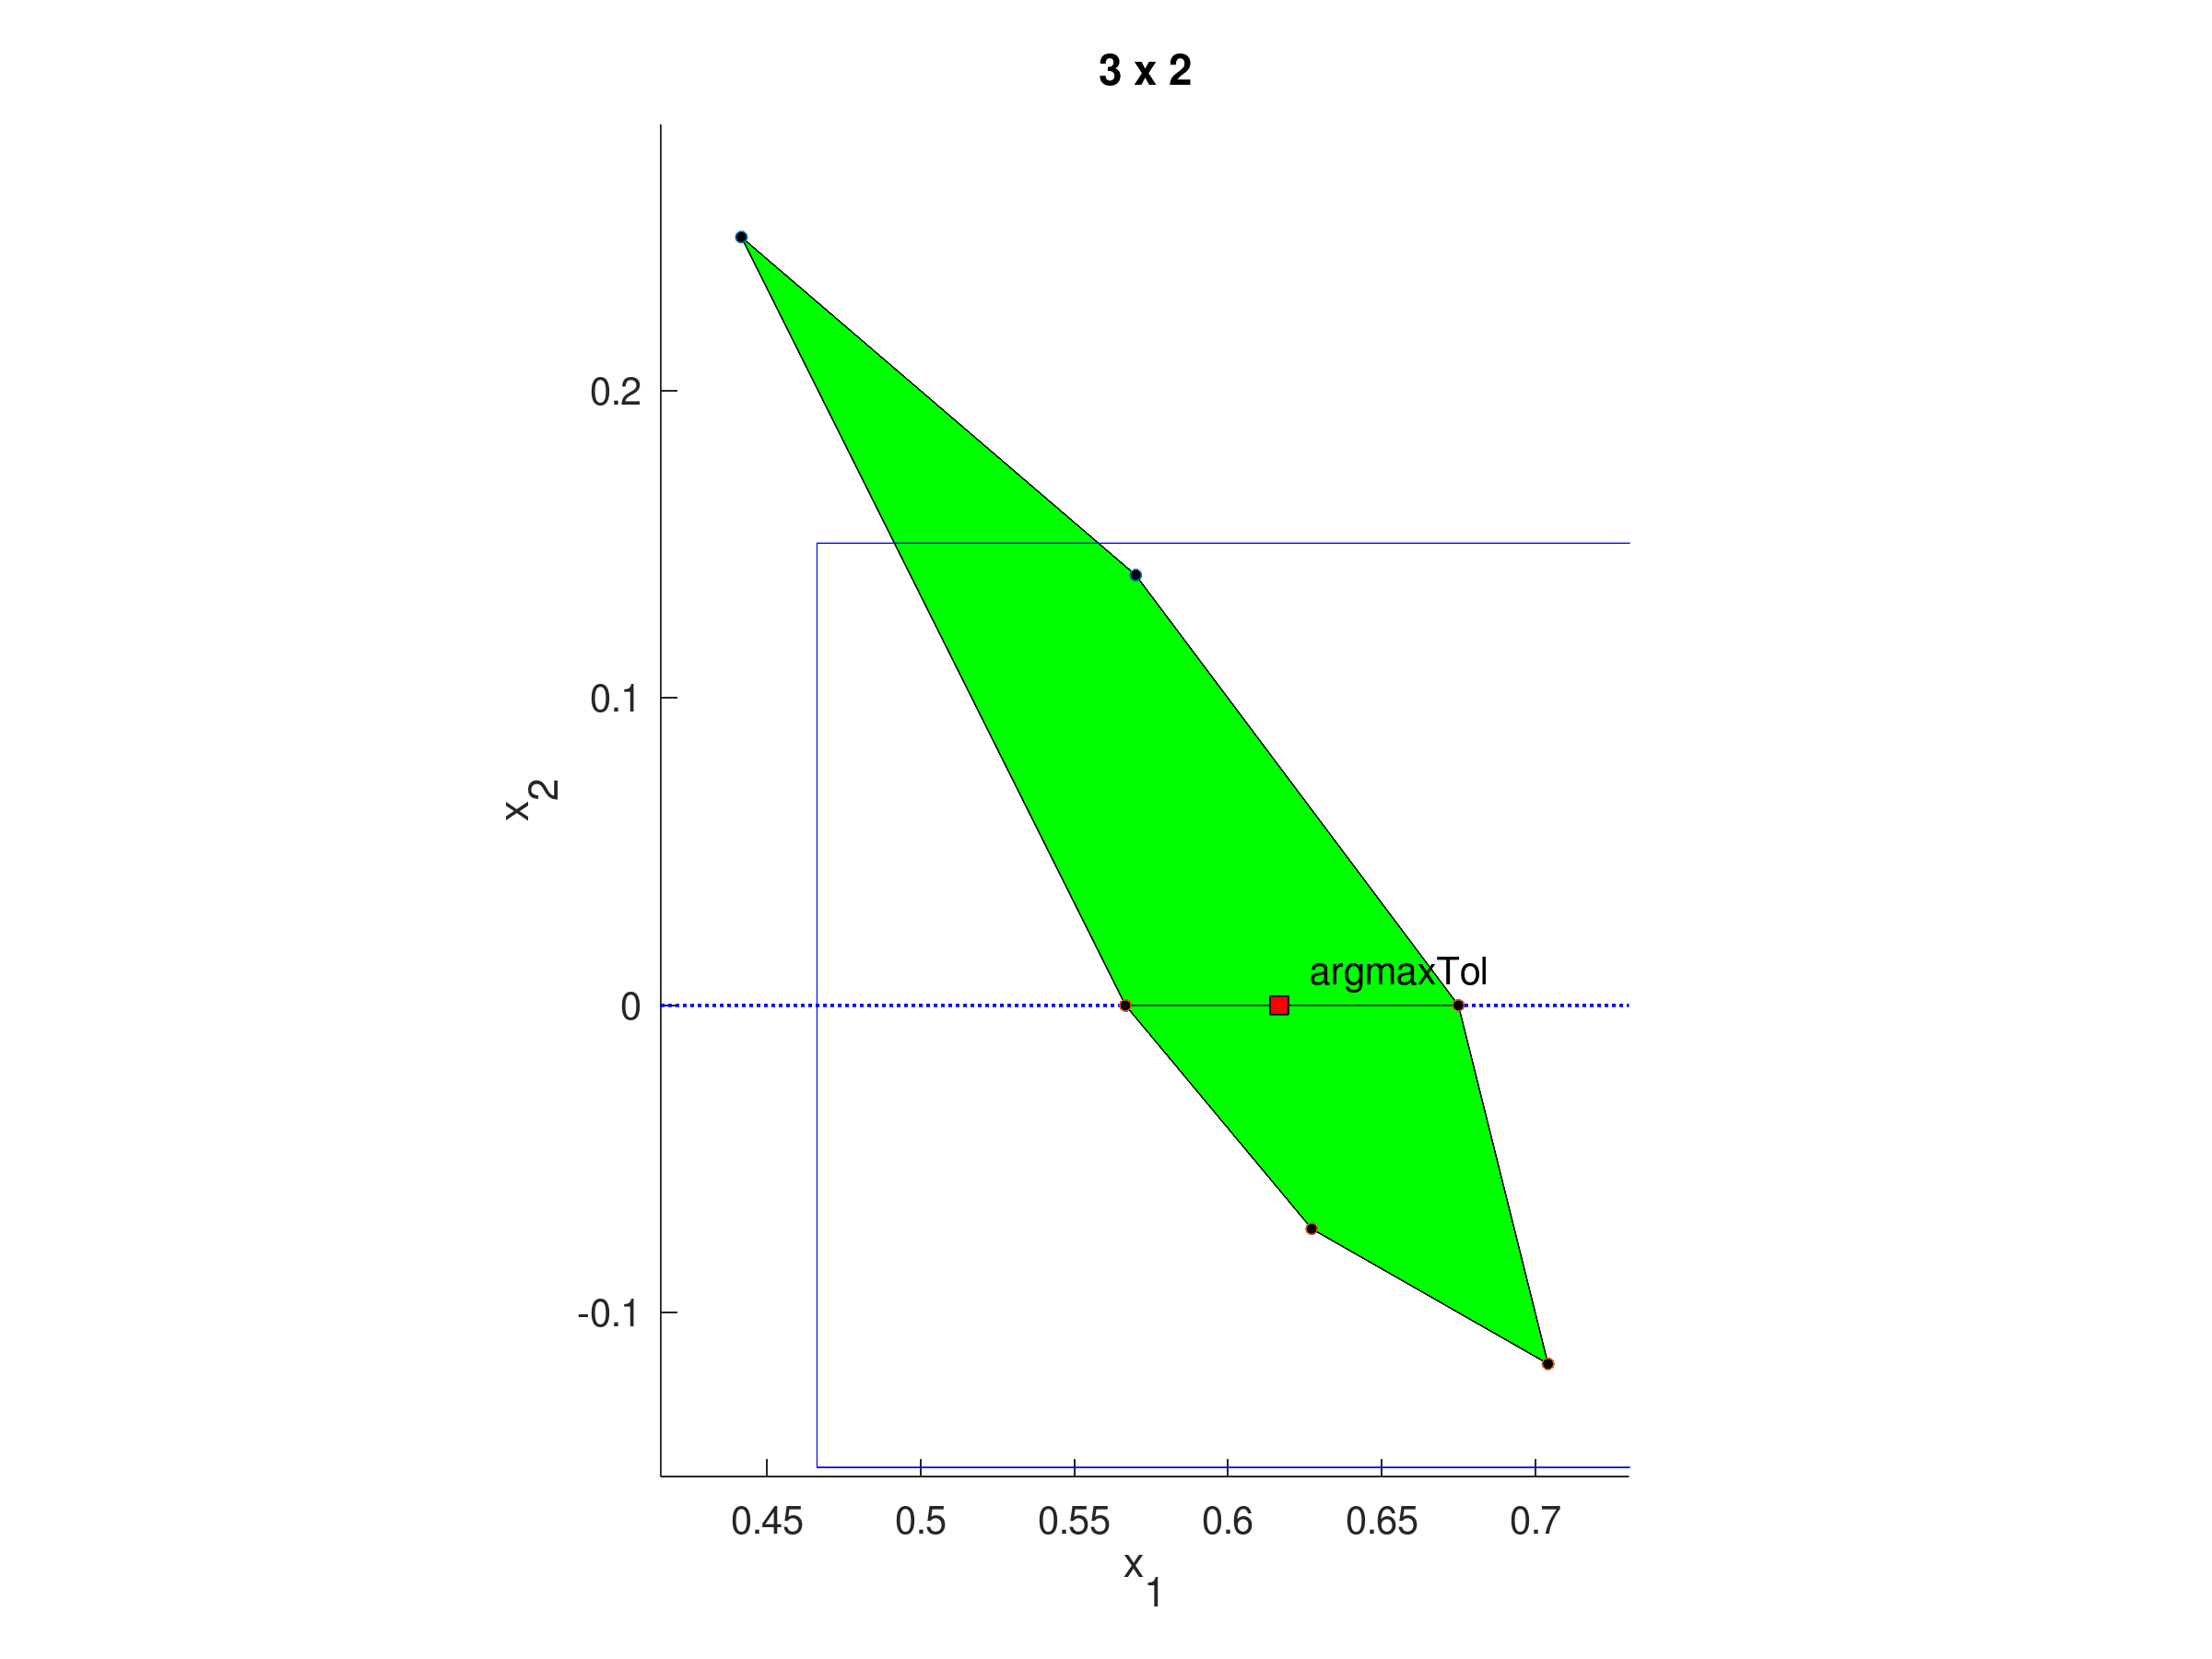
\includegraphics[scale=0.25]{3x2}
		\label{pic:32tol}
		\caption{Задача $3 \times 2$. $\Xi_{tol}$}
	\end{center}
\end{figure}

Оценка вариабельности решения: $\textrm{ive} \approx 0.30$.

\subsection{Задача $2 \times 3$}
На следующих рисунках показаны трёхмерный образ и его проекция в плоскости $Ox_1x_2$ допускового множества решения для задачи $2 \times 3$. Кроме того, показан квадрат с центром в точке максимума распознающего функционала ширины ive:

\begin{figure}[H]
	\begin{center}
		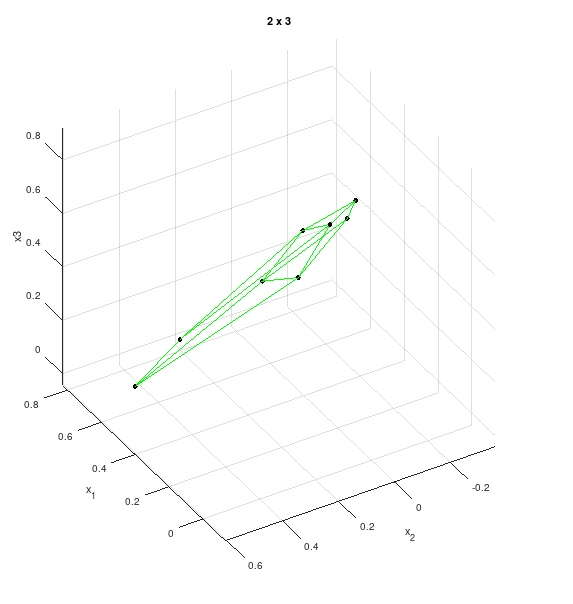
\includegraphics[scale=0.8]{2x3}
		\label{pic:23tol}
		\caption{Задача $2 \times 3$. $\Xi_{tol}$}
	\end{center}
\end{figure}

\begin{figure}[H]
	\begin{center}
		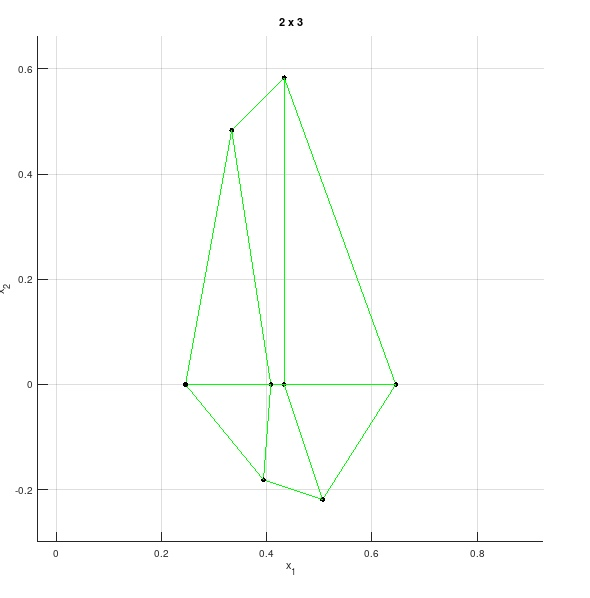
\includegraphics[scale=0.8]{2x3proj}
		\label{pic:23projtol}
		\caption{Задача $2 \times 3$. Проекция $\Xi_{tol}$ на $Ox_1x_2$}
	\end{center}
\end{figure}

Оценка вариабельности решения: $\textrm{ive} = 0.49$.